\chapter{Complex Numbers}
A simple algebraic equation like $x^{2}=-1$ may not have a real solution. Introducing complex numbers validates the existence of 'root' for every polynomial with a positive degree . Which then proves the fundamental theorem of algebra. The idea of complex numbers are widely used in Physics and Mathematics.
\begin{definition}
	A number of the form {${x+i y}$} , where $x$ and $y$ are real numbers and $i=\sqrt{(-1)},$ is called a complex number.
\end{definition}
	\textbf{\large Real Part\ \hspace{1.08cm}:} $x$ is called the real part of the complex number,  $x+i y$ and is written as,\ ${{R(x+i y)}}$.\\\\ 
	\textbf{\large Imaginary Part\ :} $y$ is called the imaginary part of the complex number and is written as,\ ${I(x+i y)}$.
	\section{Representation of a Complex number}
The point whose cartesian coordinates are $(x, y)$ uniquely
represents the complex number, {${z=x+i y}$} on the complex plane $z$. The diagram in which this representation is carried out is called the Argand's diagram. It's shown in the figure \ref{Argand Diagram}.  Since $x$ is the real part of $z$ we call the $x$ -axis the real axis. Likewise, the $y$ -axis is the imaginary axis.

		\begin{figure}[H]
				\begin{center}
			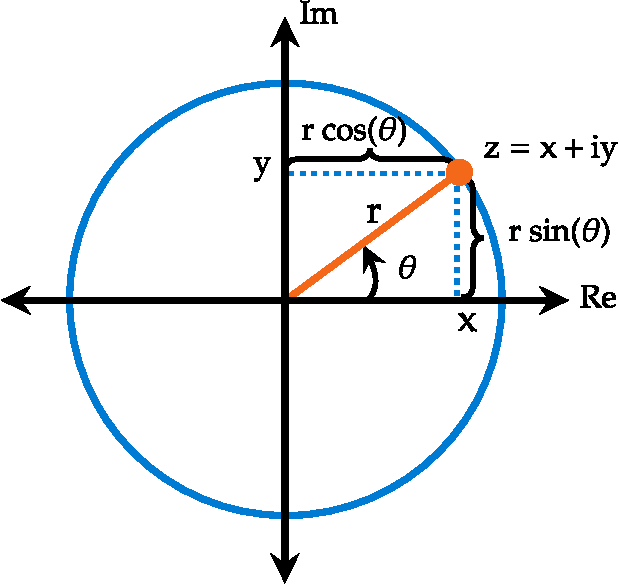
\includegraphics[width=0.30\textwidth]{cn1}
				\end{center}
			\caption{Argand Diagram}
			\label{Argand Diagram}
	    \end{figure}
    In terms of the polar coordinates  , we have
    \begin{align}
    x&=r \cos \theta, \quad y=r \sin \theta\\
    z&=x+\text { iy }=re^{i\theta} \notag \\&=r(\cos \theta+i \sin \theta)
    \label{Euler's equation}
    \end{align}
    Then, the  equation \ref{Euler's equation} is known as, Euler's formula
    \begin{figure}[H]
    	\begin{minipage}{0.40\textwidth}
    		\begin{center}
    		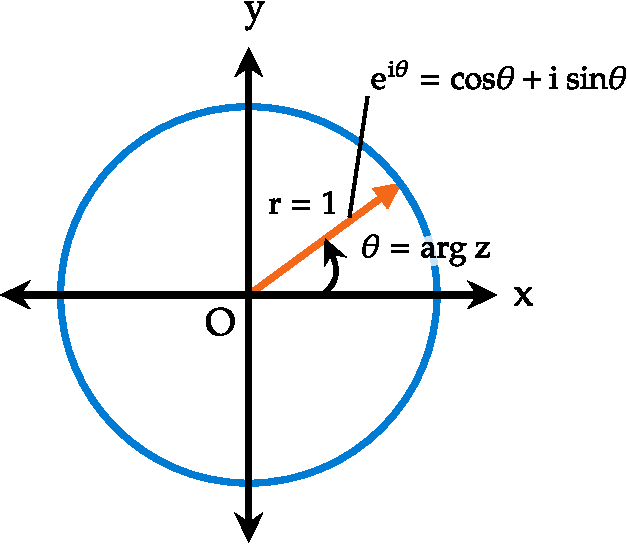
\includegraphics[width=0.70\textwidth]{cn2}
    	\end{center}
    	\end{minipage}\hfil
    	\begin{minipage}{0.40\textwidth}
    	\begin{center}
    		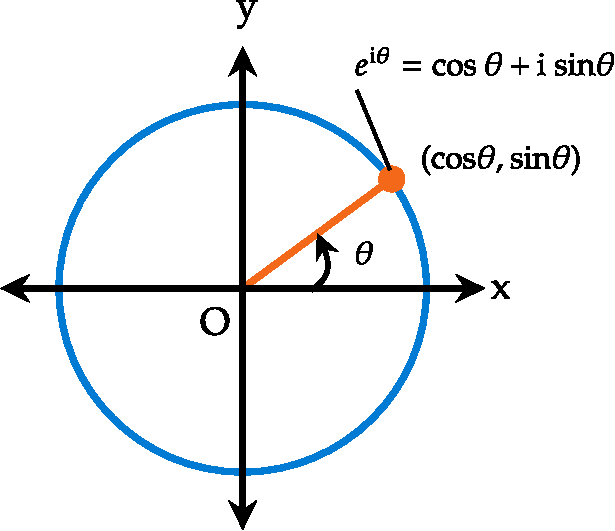
\includegraphics[width=0.70\textwidth]{cn3}
    	\end{center}
    \end{minipage}
    
    \caption{Polar representation}
    \end{figure}
   \subsection{Absolute Value}
    We define the absolute value of a complex number $x+i y$ to be the length ${r}$ of the vector from the origin to $P(x, y)$. 
    $$
    r=|x+i y|=\sqrt{x^{2}+y^{2}}
    $$
    \\\textbf{Properties:}
    \begin{itemize}
    	\item $\left|z_{1}+z_{2}\right| \leq\left|z_{1}\right|+\left|z_{2}\right|$
    	\item $\left|z_{1}-z_{2}\right| \geq\left|z_{1}\right|-\left|z_{2}\right|$
    	\item $\left|z_{1} z_{2}\right|=\left|z_{1}\right|\left|z_{2}\right|$
    	\item $\left|\frac{z_{1}}{z_{2}}\right|=\frac{\left|z_{1}\right|}{\left|z_{2}\right|}$
    \end{itemize}
    \subsection{Argument of $\mathbf{z}$ }
    The polar angle $\theta$ is called the {argument} of $z$ and it is written as, $${\theta=\arg z }$$ Any integer multiple of $2 \pi$ may be added to $\theta$ to produce another appropriate  angle.\\From the figure \ref{Argand Diagram},
    $${\theta=\arg z }=\tan ^{-1}\left(\frac{y}{x}\right)$$
    \\\textbf{Properties:}
    \begin{itemize}
    	\item $\operatorname{Arg}\left(z_{1}  z_{2} \cdot z_{3} \ldots \ldots z_{n}\right)=\operatorname{Arg} \left(z_{1}\right)+\operatorname{Arg}  \left(z_{2}\right)+\operatorname{Arg}  \left(z_{3}\right)+\ldots \ldots . .+\operatorname{Arg}\left(z_{n}\right)$
    	\item $\operatorname{Arg}\left(\frac{z_{1}}{z_{2}}\right)=\operatorname{Arg}\left(z_{1}\right)-\operatorname{Arg}\left(z_{2}\right)$
    \end{itemize}
\begin{exercise}
	Find the modulus and principal argument of the complex number
	$\frac{1+2 i}{1-(1-i)^{2}}$
\end{exercise}
\begin{answer}
	\begin{align*}
	\frac{1+2 i}{1-(1-i)^{2}}&=\frac{1+2 i}{1-(1-1-2 i)}=\frac{1+2 i}{1+2 i}\\&=1=1+0 i \\
	\therefore \quad\left|\frac{1+2 i}{1-(1-i)^{2}}\right|&=|1+0 i|=\sqrt{1^{2}}=1\\
	\text{Principal argument of}\ \frac{1+2 i}{1-(1-i)^{2}}&= \text{Principal argument of} \quad \left( 1+0 i\right) \\
	\tan ^{-1} \frac{0}{1}&=\tan ^{-1} 0\\&=0^{\circ}
	\end{align*}
\end{answer}

     \subsection{Conjugate of a Complex number}
	The conjugate of a complex number $z$ is represented by, $${\bar{z}=x-i y}$$
	\begin{note}\newline 
	$ \left. \right. $ \hspace{1.5cm}	$\begin{aligned}
		\frac{z + \bar{z}}{2}&=Re\left\lbrace z\right\rbrace \\
		\frac{z - \bar{z}}{2i}&=Im\left\lbrace z\right\rbrace\\
		z \cdot \bar{z}&=|z|^{2}
		\end{aligned}$
	\end{note}

\section{Algebra of Complex numbers}
For two Complex numbers, $a+i b$ and $c+i d $
\subsubsection{Equality:}
	\begin{align*}
	a+i b&=c+i d \quad
	\end{align*}
	Two complex numbers $(a, b)$
 and $(c, d)$ are equal if and only $a=c$ and $b=d$.
 \subsubsection{Addition:} 
 \begin{align*}
 (a+i b)+(c+i d) \quad&=(a+c)+i(b+d) \quad
 \end{align*}
 \subsubsection{Multiplication:} \begin{align*}
 (a+i b)(c+i d) &=(a c-b d)+i(a d+b c) \\
 c(a+i b)&=a c+i(b c)
 \end{align*}
 \textbf{Polar form:} 
 \begin{align*} 
 \text{Let,} \quad z_{1}&=r_{1}\left(\cos \theta_{1}+i \sin \theta_{1}\right) \quad \text{and}\quad z_{2}=r_{2}\left(\cos \theta_{2}+i \sin \theta_{2}\right)\\
 z_{1} . z_{2} &=r_{1} r_{2}\left(\cos \theta_{1}+i \sin \theta_{1}\right)\left(\cos \theta_{2}+i \sin \theta_{2}\right) \\ &=r_{1} r_{2}\left[\cos \theta_{1} \cos \theta_{2}-\sin \theta_{1} \sin \theta_{2}+i\left(\sin \theta_{1} \cos \theta_{2}+\cos \theta_{1} \sin \theta_{2}\right)\right] \\ &=r_{1} r_{1}\left[\cos \left(\theta_{1}+\theta_{2}\right)+i \sin \left(\theta_{1}+\theta_{2}\right)\right], \end{align*}
 
 \subsubsection{Division:}\begin{align*}
 \frac{c+i d}{a+i b}&=\frac{(c+i d)(a-i b)}{(a+i b)(a-i b)}\\&=\frac{(a c+b d)+i(a d-b c)}{a^{2}+b^{2}}\\
 \text{Where,}\quad x&=\frac{a c+b d}{a^{2}+b^{2}},\quad \text{and} \quad y=\frac{a d-b c}{a^{2}+b^{2}}
 \end{align*}
 \textbf{Polar form:}\\ Let $z_{1}=r_{1}\left(\cos \theta_{1}+i \sin \theta_{1}\right)$ and $z_{2}=r_{2}\left(\cos \theta_{2}+i \sin \theta_{2}\right)$\\\\\\
 $\begin{aligned} \frac{z_{1}}{z_{2}} &=\frac{r_{1}\left(\cos \theta_{1}+i \sin \theta_{1}\right)}{r_{2}\left(\cos \theta_{2}+i \sin \theta_{2}\right)}\\\\&=\frac{r_{1}\left(\cos \theta_{1}+i \sin \theta_{1}\right)\left(\cos \theta_{2}-i \sin \theta_{2}\right)}{r_{2}\left(\cos \theta_{2}+i \sin \theta_{2}\right)\left(\cos \theta_{2}-i \sin \theta_{2}\right)} \\\\ &=\frac{r_{1}\left[\left(\cos \theta_{1} \cos \theta_{2}+\sin \theta_{1} \sin \theta_{2}\right)+i\left(\sin \theta_{1} \cos \theta_{2}-\sin \theta_{2} \cos \theta_{1}\right)\right]}{r_{2}\left(\cos ^{2} \theta_{2}+\sin ^{2} \theta_{2}\right)} \\ &=\frac{r_{1}}{r_{2}}\left[\cos \left(\theta_{1}-\theta_{2}\right)+i \sin \left(\theta_{1}-\theta_{2}\right)\right] \end{aligned}$
\begin{exercise}
	Find
	\begin{enumerate}
		\item $(2+3 i)+(6-2 i)$
		\item $(2+3 i)-(6-2 i) $
		\item $(2+3 i)(6-2 i)$
		\item $\frac{2+3 i}{6-2 i}$
	\end{enumerate}
\end{exercise}
\begin{answer}\hspace{0.5cm}
		\begin{enumerate}
		\item $(2+3 i)+(6-2 i)=(2+6)+(3-2) i=8+i $
		
		\item $(2-6)+(3-(-2)) i=-4+5 i $
		\item
		\begin{align*}
		(2+3 i)(6-2 i)&=(2)(6)+(2)(-2 i)+(3 i)(6)+(3 i)(-2 i)\\
		&=12-4 i+18 i-6 i^{2}\\&=12+14 i+6=18+14 i
		\end{align*}
		\item 
		\begin{align*}
		\frac{2+3 i}{6-2 i}&=\frac{2+3 i}{6-2 i} \frac{6+2 i}{6+2 i}\\
		&=\frac{12+4 i+18 i+6 i^{2}}{36+12 i-12 i-4 i^{2}}\\
		&=\frac{6+22 i}{40}\\&=\frac{3}{20}+\frac{11}{20} i
		\end{align*}
	\end{enumerate}
\end{answer}
\begin{exercise}
	Express $\frac{(6+i) \cdot(2-i)}{(4+3 i) \cdot(1-2 i)}$ in the form of $a+i b$
\end{exercise}
\begin{answer}
	\begin{align*} \frac{(6+i) \cdot(2-i)}{(4+3 i) \cdot(1-2 i)} &=\frac{12+1+i(2-6)}{4+6+i(3-8)}=\frac{13-4 i}{10-5 i} \\ &=\frac{(13-4 i)(10+5 i)}{(10-5 i)(10+5 i)}=\frac{150+25 i}{100+25}\\&=\frac{6+i}{5}\\&=\frac{6}{5}+\frac{1}{5} i \end{align*}
\end{answer}


\section{Important Identities}
\subsection{Circular functions of Complex numbers}

\begin{align*}
	\bullet\quad\sin \theta=\frac{e^{i \theta}-e^{-i \theta}}{2 i}\quad\bullet&\quad\cos \theta=\frac{e^{i \theta}+e^{-i \theta}}{2}\\\\
\bullet\quad\sin z=\frac{e^{i z}-e^{-i z}}{2 i}\quad\bullet&\quad\cos z=\frac{e^{i z}+e^{-i z}}{2}
\end{align*}

\subsection{Hyperbolic functions of Complex numbers}
\begin{alignat*}{2}
&\bullet\quad \sinh x=\frac{e^{x}-e^{-x}}{2}\quad&&\bullet\quad \cosh x=\frac{e^{x}+e^{-x}}{2}\\
&\bullet\quad\tanh x=\frac{e^{x}-e^{-x}}{e^{x}+e^{-x}}\quad&&\bullet \quad {\coth} x=\frac{e^{x}+e^{-x}}{e^{x}-e^{-x}}
\\
&\bullet\quad{\operatorname{sech}} x=\frac{2}{e^{x}+e^{-x}} \quad&&\bullet \quad {\operatorname{cosech}} x=\frac{2}{e^{x}-e^{-x}}\\
&\bullet\quad\cosh x+\sinh x=\frac{e^{x}+e^{-x}}{2}+\frac{e^{x}-e^{-x}}{2}=e^{x} \quad&& \quad
\end{alignat*}
\begin{note}
\textbf{\textbf{Relation between Circular and Hyperbolic functions:}}\\\\
$\begin{array}{ll}\bullet\quad\sin i x=i \sinh x & \bullet\quad \sinh i x=i \sin x \\ \bullet\quad\cos i x=\cosh x & \bullet\quad \cosh i x=\cos x \\ \bullet\quad\tan i x=i \tanh x& \bullet\quad \tanh i x=i \tan x\end{array}$

\end{note}

\begin{theorem}
	\textbf{De Moivre's Theorem:}
	\begin{enumerate}
		\item For any integer $n,$ $(\cos \theta+i \sin \theta)^{n}=\cos n \theta+i \sin n \theta$
		\item 	If $n$ is a fraction, then $(\cos n \theta+i \sin n \theta)$ is one of the values .
	\end{enumerate}
\end{theorem}
\begin{exercise}
  Express $\frac{(\cos \theta+i \sin \theta)^{8}}{(\sin \theta+i \cos \theta)^{4}}$ in the form $(x+i y)$
\end{exercise}
\begin{answer}
	$$
	\begin{aligned}
	\frac{(\cos \theta+i \sin \theta)^{8}}{(\sin \theta+i \cos \theta)^{4}}=&\frac{(\cos \theta+i \sin \theta)^{8}}{(i)^{4}\left(\cos \theta+\frac{1}{i} \sin \theta\right)^{4}} \\
	=& \frac{(\cos \theta+i \sin \theta)^{8}}{(\cos \theta-i \sin \theta)^{4}}=\frac{(\cos \theta+i \sin \theta)^{8}}{[\cos (-\theta)+i \sin (-\theta)]^{4}} \\
	=& \frac{(\cos \theta+i \sin \theta)^{8}}{\left[(\cos \theta+i \sin \theta)^{-1}\right]^{4}}=\frac{(\cos \theta+i \sin \theta)^{8}}{(\cos \theta+i \sin \theta)^{-4}}=(\cos \theta+i \sin \theta)^{12} \\
	=& \cos 12 \theta+i \sin 12 \theta
	\end{aligned}
	$$
\end{answer}
\begin{note}
	Series expansion of different functions
	
	\begin{align*}
	e^{x}&=1+x+\frac{x^{2}}{2 !}+\frac{x^{3}}{3 !}+\frac{x^{4}}{4 !}+\ldots \\
	\sin x&=x-\frac{x^{3}}{3 !}+\frac{x^{5}}{5 !}-\frac{x^{7}}{7 !}+\ldots \\
	\cos x&=1-\frac{x^{2}}{2 !}+\frac{x^{4}}{4 !}-\frac{x^{6}}{6 !}+\ldots \\
	\tan x&=x+\frac{x^{3}}{3}+\frac{2 x^{5}}{15}+\frac{17 x^{7}}{315}+\frac{62 x^{9}}{2835} +\cdots\\
	\ln (1+x)&=x-\frac{x^{2}}{2}+\frac{x^{3}}{3}-\frac{x^{4}}{4}+\ldots \\
    \tan ^{-1}(x)&=x-\frac{x^{3}}{3}+\frac{x^{5}}{5}-\frac{x^{7}}{7}+\ldots
	\end{align*}
	
\end{note}
\newpage
\begin{abox}
	Practise Set-1
	\end{abox}
\begin{enumerate}[label=\color{ocre}\textbf{\arabic*.}]
	\item The value of the integral $\int_{C} d z z^{2} e^{z}$, where $C$ is an open contour in the complex $z$-plane as shown in the figure below, is:
	{\exyear{NET/JRF(JUNE-2011)}}
	\begin{figure}[H]
		\centering
		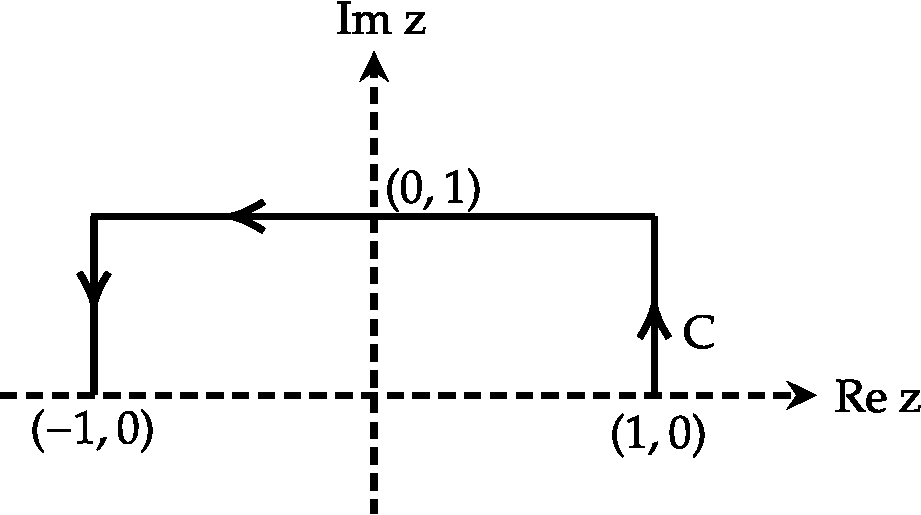
\includegraphics[height=5cm,width=9cm]{diagram-20211005-crop}
	\end{figure}
	\begin{tasks}(4)
		\task[\textbf{A.}] $\frac{5}{e}+e$
		\task[\textbf{B.}] $e-\frac{5}{e}$
		\task[\textbf{C.}] $\frac{5}{e}-e$
		\task[\textbf{D.}] $-\frac{5}{e}-e$
	\end{tasks}
	\item Which of the following is an analytic function of the complex variable $z=x+i y$ in the domain $|z|<2 ?$
	{\exyear{NET/JRF(JUNE-2011)}}
	\begin{tasks}(2)
		\task[\textbf{A.}] $(3+x-i y)^{7}$
		\task[\textbf{B.}] $(1+x+i y)^{4}(7-x-i y)^{3}$
		\task[\textbf{C.}] $(1-x-i y)^{4}(7-x+i y)^{3}$
		\task[\textbf{D.}] $(x+i y-1)^{1 / 2}$
	\end{tasks}
	\item The first few terms in the Laurent series for $\frac{1}{(z-1)(z-2)}$ in the region $1 \leq|z| \leq 2$ and around $z=1$ is
	{\exyear{NET/JRF(JUNE-2012)}}
	\begin{tasks}(1)
		\task[\textbf{A.}] $\frac{1}{2}\left[1+z+z^{2}+\ldots\right]\left[1+\frac{z}{2}+\frac{z^{2}}{4}+\frac{z^{3}}{8}+\ldots .\right]$
		\task[\textbf{B.}] $\frac{1}{1-z}-z-(1-z)^{2}+(1-z)^{3}+\ldots .$
		\task[\textbf{C.}] $\frac{1}{\mathrm{z}^{2}}\left[1+\frac{1}{\mathrm{z}}+\frac{1}{\mathrm{z}^{2}}+\ldots .\right]\left[1+\frac{2}{\mathrm{z}}+\frac{4}{\mathrm{z}^{2}}+\ldots . .\right]$
		\task[\textbf{D.}]  $2(z-1)+5(z-1)^{2}+7(z-1)^{3}+\ldots$
	\end{tasks}
	\item Let $u(x, y)=x+\frac{1}{2}\left(x^{2}-y^{2}\right)$ be the real part of analytic function $f(z)$ of the complex variable $z=x+i y$. The imaginary part of $f(z)$ is
	{\exyear{NET/JRF(JUNE-2012)}}
	\begin{tasks}(4)
		\task[\textbf{A.}] $y+x y$
		\task[\textbf{B.}] $x y$
		\task[\textbf{C.}] $y$
		\task[\textbf{D.}] $y^{2}-x^{2}$
	\end{tasks}
	\item The value of the integral $\int_{C} \frac{z^{3} d z}{\left(z^{2}-5 z+6\right)}$, where $C$ is a closed contour defined by the equation $2|z|-5=0$, traversed in the anti-clockwise direction, is
	{\exyear{NET/JRF(DEC-2012)}}
	\begin{tasks}(4)
		\task[\textbf{A.}] $-16 \pi i$
		\task[\textbf{B.}] $16 \pi \mathrm{i}$
		\task[\textbf{C.}] $8 \pi i$
		\task[\textbf{D.}] $2 \pi i$
	\end{tasks}
	\item  With $z=x+i y$, which of the following functions $f(x, y)$ is NOT a (complex) analytic function of $z$ ?
	{\exyear{NET/JRF(JUNE-2013)}}
	\begin{tasks}(1)
		\task[\textbf{A.}] $f(x, y)=(x+i y-8)^{3}\left(4+x^{2}-y^{2}+2 i x y\right)^{7}$
		\task[\textbf{B.}] $f(x, y)=(x+i y)^{7}(1-x-i y)^{3}$
		\task[\textbf{C.}] $f(x, y)=\left(x^{2}-y^{2}+2 i x y-3\right)^{5}$
		\task[\textbf{D.}] $f(x, y)=(1-x+i y)^{4}(2+x+i y)^{6}$
	\end{tasks}
	\item  Which of the following functions cannot be the real part of a complex analytic function of $z=x+i y ?$
	{\exyear{NET/JRF(DEC-2013)}}
	\begin{tasks}(4)
		\task[\textbf{A.}] $x^{2} y$
		\task[\textbf{B.}]  $x^{2}-y^{2}$
		\task[\textbf{C.}] $x^{3}-3 x y^{2}$
		\task[\textbf{D.}] $3 x^{2} y-y-y^{3}$
	\end{tasks}
	\item  Given that the integral $\int_{0}^{\infty} \frac{d x}{y^{2}+x^{2}}=\frac{\pi}{2 y}$, the value of $\int_{0}^{\infty} \frac{d x}{\left(y^{2}+x^{2}\right)^{2}}$ is
	{\exyear{NET/JRF(DEC-2013)}}
	\begin{tasks}(4)
		\task[\textbf{A.}] $\frac{\pi}{y^{3}}$
		\task[\textbf{B.}] $\frac{\pi}{4 y^{3}}$
		\task[\textbf{C.}]  $\frac{\pi}{8 y^{3}}$
		\task[\textbf{D.}] $\frac{\pi}{2 y^{3}}$
	\end{tasks}
	\item If $C$ is the contour defined by $|z|=\frac{1}{2}$, the value of the integral
	$$
	\oint_{C} \frac{d z}{\sin ^{2} z}
	$$
	is
	{\exyear{NET/JRF(JUNE-2014)}}
	\begin{tasks}(4)
		\task[\textbf{A.}] $\infty$
		\task[\textbf{B.}] $2 \pi i$
		\task[\textbf{C.}] 0
		\task[\textbf{D.}] $\pi i$
	\end{tasks}
	\item The principal value of the integral $\int_{-\infty}^{\infty} \frac{\sin (2 x)}{x^{3}} d x$ is
	{\exyear{NET/JRF(DEC-2014)}}
	\begin{tasks}(4)
		\task[\textbf{A.}] $-2 \pi$
		\task[\textbf{B.}]  $-\pi$
		\task[\textbf{C.}] $\pi$
		\task[\textbf{D.}]  $2 \pi$
	\end{tasks}
	\item The Laurent series expansion of the function $f(z)=e^{2}+e^{1 / 2}$ about $z=0$ is given by
	{\exyear{NET/JRF(DEC-2014)}}
	\begin{tasks}(2)
		\task[\textbf{A.}] $\sum_{n=-\infty}^{\infty} \frac{z^{n}}{n !}$ for all $|z|<\infty$
		\task[\textbf{B.}] $\sum_{n=0}^{\infty}\left(z^{n}+\frac{1}{z^{n}}\right) \frac{1}{n !}$ only if $0<|z|<1$
		\task[\textbf{C.}] $\sum_{n=0}^{\infty}\left(z^{n}+\frac{1}{z^{n}}\right) \frac{1}{n !}$ for all $0<|z|<\infty$
		\task[\textbf{D.}]  $\sum_{n=-\infty}^{\infty} \frac{z^{n}}{n !}$ only if $|z|<1$
	\end{tasks}
	\item Consider the function $f(z)=\frac{1}{z} \ln (1-z)$ of a complex variable $z=r e^{i \theta}(r \geq 0, \quad-\infty<\theta<\infty)$. The singularities of $f(z)$ are as follows:
	{\exyear{NET/JRF(DEC-2014)}}
	\begin{tasks}(1)
		\task[\textbf{A.}]  Branch points at $z=1$ and $z=\infty$; and a pole at $z=0$ only for $0 \leq \theta<2 \pi$
		\task[\textbf{B.}] Branch points at $z=1$ and $z=\infty$; and a pole at $z=0$ for all $\theta$ other than $0 \leq \theta<2 \pi$
		\task[\textbf{C.}] Branch points at $z=1$ and $z=\infty$; and a pole at $z=0$ for all $\theta$
		\task[\textbf{D.}] Branch points at $z=0, z=1$ and $z=\infty$.
	\end{tasks}
	\item  The value of integral $\int_{-\infty}^{\infty} \frac{d x}{1+x^{4}}$
	{\exyear{NET/JRF(JUNE-2015)}}
	\begin{tasks}(4)
		\task[\textbf{A.}] $\frac{\pi}{\sqrt{2}}$
		\task[\textbf{B.}] $\frac{\pi}{2}$
		\task[\textbf{C.}] $\sqrt{2} \pi$
		\task[\textbf{D.}] $2 \pi$
	\end{tasks}
	\item  The function $\frac{Z}{\sin \pi z^{2}}$ of a complex variable $z$ has
	{\exyear{NET/JRF(DEC-2015)}}
	\begin{tasks}(1)
		\task[\textbf{A.}] A simple pole at 0 and poles of order 2 at $\pm \sqrt{n}$ for $n=1,2,3 \ldots$
		\task[\textbf{B.}] A simple pole at 0 and poles of order 2 at $\pm \sqrt{n}$ and $\pm i \sqrt{n}$ for $n=1,2,3 \ldots$
		\task[\textbf{C.}] Poles of order 2 at $\pm \sqrt{n}, n=0,1,2,3 \ldots$
		\task[\textbf{D.}] Poles of order 2 at $\pm n, n=0,1,2,3 \ldots$
	\end{tasks}
	\item The value of the contour integral $\frac{1}{2 \pi i} \oint_{C} \frac{e^{4 z}-1}{\cosh (z)-2 \sinh (z)} d z$ around the unit circle $C$ traversed in the anti-clockwise direction, is
	{\exyear{NET/JRF(JUNE-2016)}}
	\begin{tasks}(4)
		\task[\textbf{A.}] 0
		\task[\textbf{B.}] 2
		\task[\textbf{C.}] $\frac{-8}{\sqrt{3}}$
		\task[\textbf{D.}] $-\tanh \left(\frac{1}{2}\right)$
	\end{tasks}
	\item  Let $u(x, y)=e^{a x} \cos (b y)$ be the real part of a function $f(z)=u(x, y)+i v(x, y)$ of the complex variable $z=x+i y$, where $a, b$ are real constants and $a \neq 0 .$ The function $f(z)$ is complex analytic everywhere in the complex plane if and only if
	{\exyear{NET/JRF(JUNE-2017)}}
	\begin{tasks}(4)
		\task[\textbf{A.}] $b=0$
		\task[\textbf{B.}] $b=\pm a$
		\task[\textbf{C.}] $b=\pm 2 \pi a$
		\task[\textbf{D.}]  $b=a \pm 2 \pi$
	\end{tasks}
	\item  The integral $\oint_{\Gamma} \frac{z e^{i \pi z / 2}}{z^{2}-1} d z$ along the closed contour $\Gamma$ shown in the figure is
	{\exyear{NET/JRF(JUNE-2017)}}
	\begin{figure}[H]
		\centering
		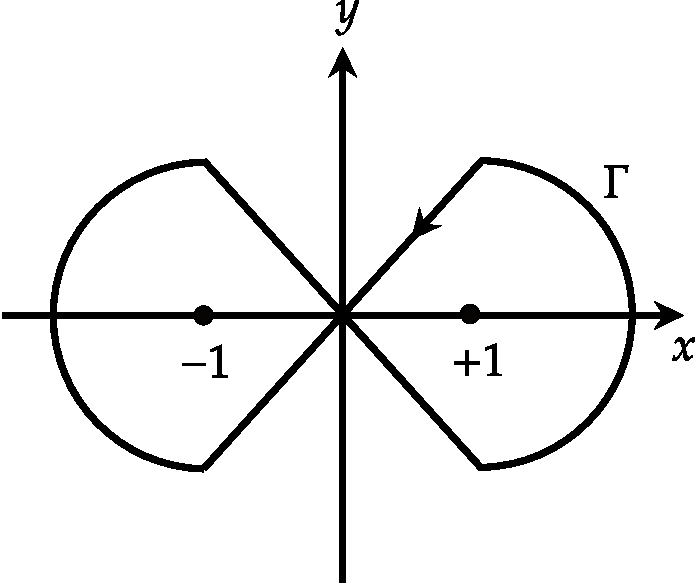
\includegraphics[height=4cm,width=5cm]{diagram-20211005(19)-crop}
	\end{figure}
	\begin{tasks}(4)
		\task[\textbf{A.}] 0
		\task[\textbf{B.}] $2 \pi$
		\task[\textbf{C.}] $-2 \pi$
		\task[\textbf{D.}] $4 \pi i$
	\end{tasks}
	\item What is the value of $a$ for which $f(x, y)=2 x+3\left(x^{2}-y^{2}\right)+2 i(3 x y+a y)$ is an analytic function of complex variable $z=x+i y$
	{\exyear{NET/JRF(JUNE-2018)}}
	\begin{tasks}(4)
		\task[\textbf{A.}] 1
		\task[\textbf{B.}] 0
		\task[\textbf{C.}] 3
		\task[\textbf{D.}] 2
	\end{tasks}
\item  The value of the integral $\oint_{C} \frac{d z}{z} \frac{\tanh 2 z}{\sin \pi z}$, where $C$ is a circle of radius $\frac{\pi}{2}$, traversed counter-clockwise, with centre at $z=0$, is
{\exyear{NET/JRF(DEC-2018)}}
\begin{tasks}(4)
	\task[\textbf{A.}] 4
	\task[\textbf{B.}] $4 i$
	\task[\textbf{C.}] $2 i$
	\task[\textbf{D.}] 0
\end{tasks}
	\item The integral $I=\int_{C} e^{z} d z$ is evaluated from the point $(-1,0)$ to $(1,0)$ along the contour $C$, which is an arc of the parabola $y=x^{2}-1$, as shown in the figure. The value of $I$ is
	{\exyear{NET/JRF(DEC-2018)}}
	\begin{figure}[H]
		\centering
		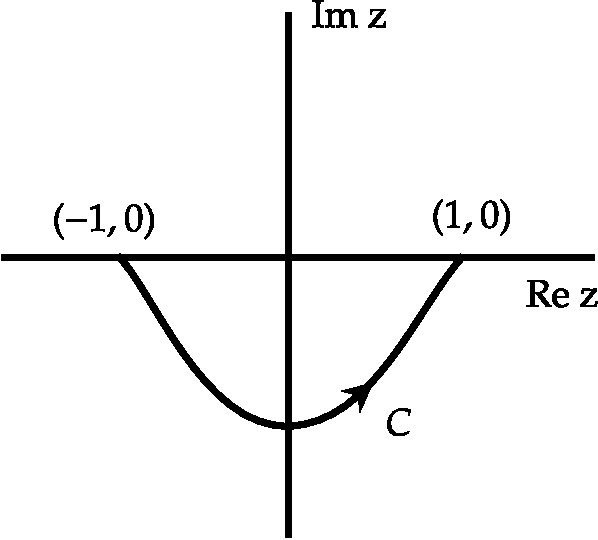
\includegraphics[height=4.5cm,width=5cm]{diagram-20211005(3)-crop}
	\end{figure}
	\begin{tasks}(4)
		\task[\textbf{A.}]  0
		\task[\textbf{B.}] $2 \sinh 1$
		\task[\textbf{C.}]  $e^{2 i} \sinh 1$
		\task[\textbf{D.}] $e+e^{-1}$
	\end{tasks}
	\item The contour $C$ of the following integral
	$$
	\oint_{C} d z \frac{\sqrt{(z-1)(z-3)}}{\left(z^{2}-25\right)^{3}}
	$$
	in the complex $z$ plane is shown in the figure below.\\
	\begin{figure}[H]
		\centering
		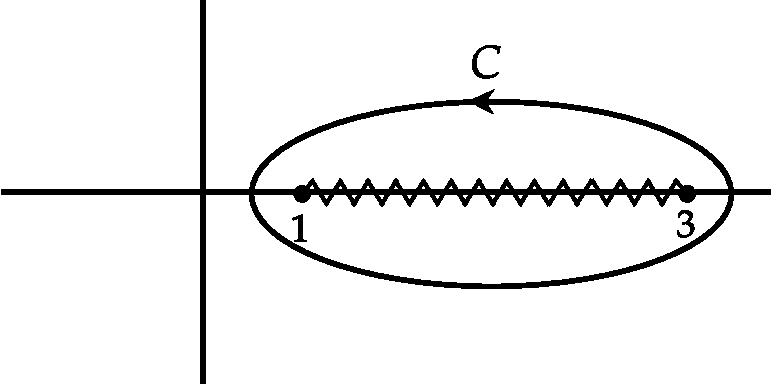
\includegraphics[height=3.5cm,width=6cm]{diagram-20211005(8)-crop}
	\end{figure}
	This integral is equivalent to an integral along the contours
	{\exyear{NET/JRF(DEC-2018)}}
	\begin{tasks}(2)
		\task[\textbf{A.}] \begin{figure}[H]
			\centering
			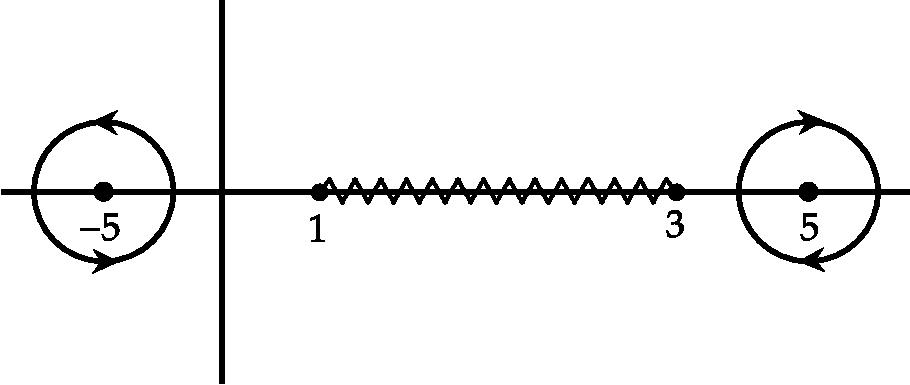
\includegraphics[height=3cm,width=6.5cm]{diagram-20211005(4)-crop}
		\end{figure}
		\task[\textbf{B.}] \begin{figure}[H]
			\centering
			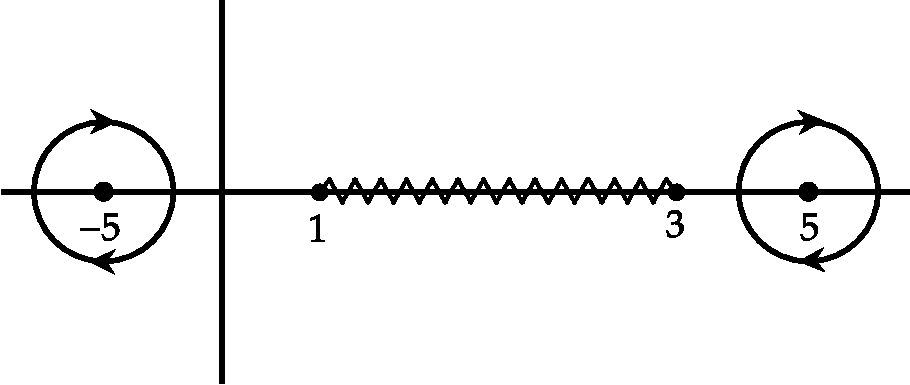
\includegraphics[height=3cm,width=6.5cm]{diagram-20211005(5)-crop}
		\end{figure}
		\task[\textbf{C.}] \begin{figure}[H]
			\centering
			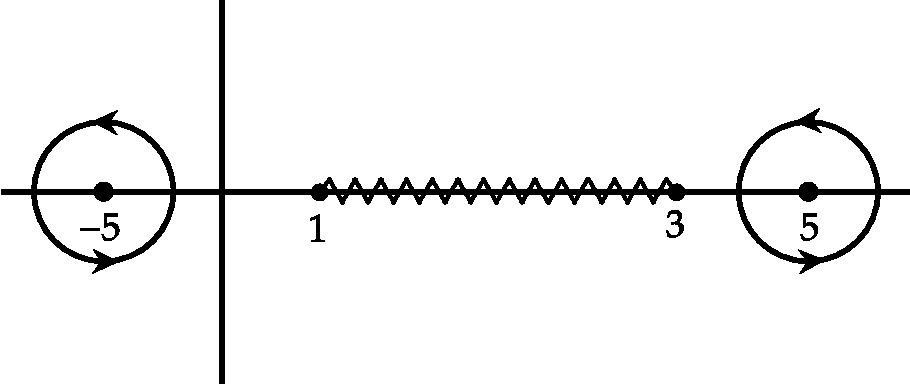
\includegraphics[height=3cm,width=6.5cm]{diagram-20211005(6)-crop}
		\end{figure}
		\task[\textbf{D.}] \begin{figure}[H]
			\centering
			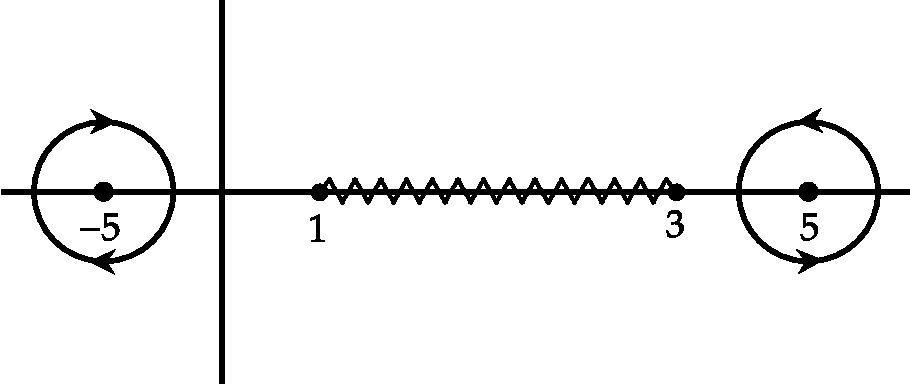
\includegraphics[height=3cm,width=6.5cm]{diagram-20211005(7)-crop}
		\end{figure}
	\end{tasks}
	\item  Let $C$ be the circle of radius $\frac{\pi}{4}$ centered at $z=\frac{1}{4}$ in the complex $z$-plane that is traversed counter-clockwise. The value of the contour integral $\oint_{C} \frac{z^{2}}{\sin ^{2} 4 z} d z$ is
	{\exyear{NET/JRF(DEC-2019)}}
	\begin{tasks}(4)
		\task[\textbf{A.}] 0
		\task[\textbf{B.}] $\frac{i \pi^{2}}{4}$
		\task[\textbf{C.}] $\frac{i \pi^{2}}{16}$
		\task[\textbf{D.}] $\frac{i \pi}{4}$
	\end{tasks}
	\item  A function of a complex variable $z$ is defined by the integral $f(z)=\oint_{\Gamma} \frac{w^{2}-2}{w-z} d w$, where $\Gamma$ is a circular contour of radius 3 , centred at origin, running counter-clockwise in the $w$ - plane. The value of the function at $z=(2-i)$ is
	{\exyear{NET/JRF(JUNE-2020)}}
	\begin{tasks}(4)
		\task[\textbf{A.}] 0
		\task[\textbf{B.}] $1-4 i$
		\task[\textbf{C.}]  $8 \pi+2 \pi \mathrm{i}$
		\task[\textbf{D.}] $-\frac{2}{\pi}-\frac{i}{2 \pi}$
	\end{tasks}
\end{enumerate}
 \colorlet{ocre1}{ocre!70!}
\colorlet{ocrel}{ocre!30!}
\setlength\arrayrulewidth{1pt}
\begin{table}[H]
	\centering
	\arrayrulecolor{ocre}
	\begin{tabular}{|p{1.5cm}|p{1.5cm}||p{1.5cm}|p{1.5cm}|}
		\hline
		\multicolumn{4}{|c|}{\textbf{Answer key}}\\\hline\hline
		\rowcolor{ocrel}Q.No.&Answer&Q.No.&Answer\\\hline
		1&\textbf{C} &2&\textbf{B}\\\hline 
		3&\textbf{B} &4&\textbf{A} \\\hline
		5&\textbf{A} &6&\textbf{D} \\\hline
		7&\textbf{A}&8&\textbf{-}\\\hline
		9&\textbf{C}&10&\textbf{A}\\\hline
		11&\textbf{C} &12&\textbf{-}\\\hline
		13&\textbf{A}&14&\textbf{B}\\\hline
		15&\textbf{C}&16&\textbf{B}\\\hline
		17&\textbf{C} &18&\textbf{A}\\\hline
		19&\textbf{B}&20&\textbf{B}\\\hline
		21&\textbf{C}&22&\textbf{C}\\\hline
		23&\textbf{C}& &\\\hline
		
	\end{tabular}
\end{table}
\newpage
\begin{abox}
	Practise Set-2
\end{abox}
\begin{enumerate}[label=\color{ocre}\textbf{\arabic*.}]
	\item  The value of the integral $\oint_{C} \frac{e^{z} \sin (z)}{z^{2}} d z$, where the contour $C$ is the unit circle: $|z-2|=1$, is
	{\exyear{GATE 2010}}
	\begin{tasks}(4)
		\task[\textbf{A.}] $2 \pi i$
		\task[\textbf{B.}] $4 \pi i$
		\task[\textbf{C.}] $\pi i$
		\task[\textbf{D.}] 0
	\end{tasks}
	\item Which of the following statements is TRUE for the function $f(z)=\frac{z \sin z}{(z-\pi)^{2}}$ ?
	{\exyear{GATE 2011}}
	\begin{tasks}(1)
		\task[\textbf{A.}] $f(z)$ is analytic everywhere in the complex plane
		\task[\textbf{B.}] $f(z)$ has a zero at $z=\pi$
		\task[\textbf{C.}] $f(z)$ has a pole of order 2 at $z=\pi$
		\task[\textbf{D.}] $f(z)$ has a simple pole at $z=\pi$
	\end{tasks}
	\item For the function $f(z)=\frac{16 z}{(z+3)(z-1)^{2}}$, the residue at the pole $z=1$ is (your answer should be an integer)-------
	{\exyear{GATE 2013}}
	\item The value of the integral
	$$
	\oint_{C} \frac{z^{2}}{e^{z}+1} d z
	$$
	where $C$ is the circle $|z|=4$, is
	{\exyear{GATE 2014}}
	\begin{tasks}(4)
		\task[\textbf{A.}] $2 \pi i$
		\task[\textbf{B.}] $2 \pi^{2} i$
		\task[\textbf{C.}]  $4 \pi^{3} i$
		\task[\textbf{D.}] $4 \pi^{2} i$
	\end{tasks}
	\item Consider a complex function $f(z)=\frac{1}{z\left(z+\frac{1}{2}\right) \cos (z \pi)}$. Which one of the following statements is correct?
	{\exyear{GATE 2015}}
	\begin{tasks}(1)
		\task[\textbf{A.}] $f(z)$ has simple poles at $z=0$ and $z=-\frac{1}{2}$
		\task[\textbf{B.}] $f(z)$ has second order pole at $z=-\frac{1}{2}$
		\task[\textbf{C.}] $f(z)$ has infinite number of second order poles
		\task[\textbf{D.}] $f(z)$ has all simple poles
	\end{tasks}
	\item  Consider $w=f(z)=u(x, y)+i v(x, y)$ to be an analytic function in a domain $D$. Which one of the following options is NOT correct?
	{\exyear{GATE 2015}}
	\begin{tasks}(1)
		\task[\textbf{A.}] $u(x, y)$ satisfies Laplace equation in D
		\task[\textbf{B.}]  $v(x, y)$ satisfies Laplace equation in $D$
		\task[\textbf{C.}] $\int_{1}^{z_{2}} f(z) d z$ is dependent on the choice of the contour between $z_{1}$ and $z_{2}$ in $D$
		\task[\textbf{D.}]  $f(z)$ can be Taylor expended in $D$
	\end{tasks}
	\item A function $y(z)$ satisfies the ordinary differential equation $y^{\prime \prime}+\frac{1}{z} y^{\prime}-\frac{m^{2}}{z^{2}} y=0$, where\\
	$m=0,1,2,3, \ldots . .$ Consider the four statements P, Q, R, S as given below.\\
	$\mathrm{P}: z^{m}$ and $z^{-m}$ are linearly independent solutions for all values of $m$\\
	Q: $z^{m}$ and $z^{-m}$ are linearly independent solutions for all values of $m>0$\\
	$\mathrm{R}$ : $\ln z$ and 1 are linearly independent solutions for $m=0$\\
	S: $z^{m}$ and $\ln z$ are linearly independent solutions for all values of $m$\\
	The correct option for the combination of valid statements is
	{\exyear{GATE 2015}}
	\begin{tasks}(4)
		\task[\textbf{A.}] P, R and S only
		\task[\textbf{B.}]  P and R only
		\task[\textbf{C.}] $\mathrm{Q}$ and $\mathrm{R}$ only
		\task[\textbf{D.}] $\mathrm{R}$ and $\mathrm{S}$ only
	\end{tasks}
	\item  Which of the following is an analytic function of $z$ everywhere in the complex plane?
	{\exyear{GATE 2016}}
	\begin{tasks}(4)
		\task[\textbf{A.}] $z^{2}$
		\task[\textbf{B.}]  $\left(z^{*}\right)^{2}$
		\task[\textbf{C.}] $|z|^{2}$
		\task[\textbf{D.}] $\sqrt{z}$
	\end{tasks}
	\item The contour integral $\oint \frac{d z}{1+z^{2}}$ evaluated along a contour going from $-\infty$ to $+\infty$ along the
	real axis and closed in the lower half-plane circle is equal to............... (up to two decimal places).
	{\exyear{GATE 2017}}
	\item The imaginary part of an analytic complex function is $v(x, y)=2 x y+3 y .$ The real part of the function is zero at the origin. The value of the real part of the function at $1+i$ is ................. (up to two decimal places)
	{\exyear{GATE 2017}}
	\item The absolute value of the integral
	$$
	\int \frac{5 z^{3}+3 z^{2}}{z^{2}-4} d z
	$$
	over the circle $|z-1.5|=1$ in complex plane, is $\ldots$ (up to two decimal places).
	{\exyear{GATE 2018}}
	\item The pole of the function $f(z)=\cot z$ at $z=0$ is
	{\exyear{GATE 2019}}
	\begin{tasks}(2)
		\task[\textbf{A.}] A removable pole
		\task[\textbf{B.}] An essential singularity
		\task[\textbf{C.}]  A simple pole
		\task[\textbf{D.}] A second order pole
	\end{tasks}
	\item The value of the integral $\int_{-\infty}^{\infty} \frac{\cos (k x)}{x^{2}+a^{2}} d x$, where $k>0$ and $a>0$, is
	{\exyear{GATE 2019}}
	\begin{tasks}(4)
		\task[\textbf{A.}] $\frac{\pi}{a} e^{-k a}$
		\task[\textbf{B.}] $\frac{2 \pi}{a} e^{-k a}$
		\task[\textbf{C.}] $\frac{\pi}{2 a} e^{-k a}$
		\task[\textbf{D.}] $\frac{3 \pi}{2 a} e^{-k a}$
	\end{tasks}
\end{enumerate}
 \colorlet{ocre1}{ocre!70!}
\colorlet{ocrel}{ocre!30!}
\setlength\arrayrulewidth{1pt}
\begin{table}[H]
	\centering
	\arrayrulecolor{ocre}
	\begin{tabular}{|p{1.5cm}|p{1.7cm}||p{1.5cm}|p{1.5cm}|}
		\hline
		\multicolumn{4}{|c|}{\textbf{Answer key}}\\\hline\hline
		\rowcolor{ocrel}Q.No.&Answer&Q.No.&Answer\\\hline
		1&\textbf{D} &2&\textbf{C}\\\hline 
		3&\textbf{3(NAT)} &4&\textbf{C} \\\hline
		5&\textbf{A} &6&\textbf{C} \\\hline
		7&\textbf{C}&8&\textbf{A}\\\hline
		9&\textbf{$\pi$(NAT)}&10&\textbf{3(NAT)}\\\hline
		11&\textbf{81.64(NAT)} &12&\textbf{C}\\\hline
		13&\textbf{A}& &\textbf{}\\\hline
		
	\end{tabular}
\end{table}
\newpage
\begin{abox}
	Practise Set-3
\end{abox}
\begin{enumerate}[label=\color{ocre}\textbf{\arabic*.}]
	\item Find the smallest positive integer $n$ for which
	$$
	\left(\frac{1+i}{1-i}\right)^{n}=1
	$$
	\begin{answer}
		\begin{align*}
		{\left[\frac{1+i}{1-i}\right]^{n}}&=1 \\
		{\left[\frac{1+i}{1-i} \times \frac{1+i}{1+i}\right]^{n}}&=1\\ \Rightarrow\left(\frac{1-1+2 i}{1+1}\right)^{n}&=1 \\
		(i)^{n}&=1=(i)^{4} \Rightarrow n=4
		\end{align*}
	
	\end{answer}
\item  Find the square root of the complex number $5+12 i$.

\begin{answer}
\begin{align}
\text{Let,}\quad \sqrt{5+12 i}&=x+i y \label{1}\\
\text{Squaring both sides of\quad \ref{1}}\quad \text{we get,}\notag\\
5+12 i=(x+i y)^{2}&=\left(x^{2}-y^{2}\right)+i 2 x y \label{2}\\
\text{Equating real and imaginary parts of \ref{2}}\notag\\
\text{we get,}\quad x^{2}-y^{2}&=5\label{3}\\
\text{and}\quad
2 x y &=12 \notag\\
x^{2}+y^{2} &=\sqrt{{({x^{2}-y^{2}})^{2}} +{4{x^{2}y^{2}}}}=\sqrt{(5)^{2}+(12)^{2}}\notag\\
&=\sqrt{25+144}=\sqrt{169}=13 \\
x^{2}+y^{2} &=13\label{4}\\
\text{adding}\quad\ref{3} \quad\text{and}\quad\ref{4}\quad\text{we get,}\notag\\
2 x^{2}=5+13=18 &\Rightarrow x=\sqrt{\frac{18}{2}}=\sqrt{9}=\pm 3\\
\text{subtracting}\quad\ref{3} \quad\text{by}\quad\ref{4}\quad\text{we get,}\notag\\
2 y^{2}=13-5=8 &\Rightarrow y=\sqrt{\frac{8}{2}}=\sqrt{4}=\pm 2\\
\text{since $ xy$ is positive,}&\text{ so $x$ and $y$ are of same sign}\notag \\
\text{Hence, $x=\pm 3, y=\pm 2$}\notag\\\therefore \sqrt{5+12 i}&=\pm 3 \pm 2 i \notag\\ i.e. \quad(3+2 i) &\text{or} -(3+2 i)\notag
\end{align}
\end{answer}
\item The value of $\frac{(\cos 3 \theta+i \sin 3 \theta)^{4}(\cos 4 \theta-i \sin 4 \theta)^{5}}{(\cos 4 \theta+i \sin 4 \theta)^{3}(\cos 5 \theta+i \sin 5 \theta)^{-4}}$ is
\begin{answer}
\begin{align*}
\text{We have, }
(\cos 3 \theta+i \sin 3 \theta)^{4}&=\cos 12 \theta+i \sin 12 \theta=(\cos \theta+i \sin \theta)^{12}\\
(\cos 4 \theta-i \sin 4 \theta)^{5}&=\cos 20 \theta-i \sin 20 \theta=(\cos \theta+i \sin \theta)^{-20} \\
(\cos 4 \theta+i \sin 4 \theta)^{3}&=\cos 12 \theta+i \sin 12 \theta=(\cos \theta+i \sin \theta)^{12}\\
(\cos 5 \theta+i \sin 5 \theta)^{-4}&=\cos 20 \theta-i \sin 20 \theta=(\cos \theta+i \sin \theta)^{-20}\\
\text{Hence the value of given expression is 1}
\end{align*}
\end{answer}
\item Write $i^{(1-i)}$ in the form $r(\cos \theta+i \sin \theta)$
\begin{answer}
	\begin{align*}
		i^{1-i} &=e^{\log i^{(1-i)}}=e^{(1-i) \log i} \\
		&=e^{(1-i) \log \left(\cos \frac{\pi}{2}+i \sin \frac{\pi}{2}\right)}\\
		&=e^{(1-i) \log \left\{\cos \left(2 n \pi+\frac{\pi}{2}\right)+i \sin \left(2 n \pi+\frac{\pi}{2}\right)\right\}} \\
		&=e^{(1-i)} \log e^{i\left(2 n \pi+\frac{\pi}{2}\right)} \\
		&=e^{(1-i) i\left(2 n \pi+\frac{\pi}{2}\right)}=e^{(i+1)\left(2 n \pi+\frac{\pi}{2}\right)} \\
		&=e^{i\left(2 n \pi+\frac{\pi}{2}\right)} \cdot e^{\left(2 n \pi+\frac{\pi}{2}\right)} \\
		&=\mathrm{e}^{\left(2 n \pi+\frac{\pi}{2}\right)}\left\{\cos \left(2 n \pi+\frac{\pi}{2}\right)+i \sin \left(2 n \pi+\frac{\pi}{2}\right)\right\} \\
		&=e^{\left(2 n \pi+\frac{\pi}{2}\right)} . i=i e^{\left(2 n \pi+\frac{\pi}{2}\right)}
	\end{align*}
\end{answer}
\item Find the general value of $\log (1+i)+\log (1-i)$
\begin{answer}
	\begin{align*}
	1+i&=\sqrt{2}\left(\frac{1}{\sqrt{2}}+\frac{i}{\sqrt{2}}\right)\\
		&=\sqrt{2}\left\{\cos \left(2 n+\frac{1}{4}\right) \pi+i \sin \left(2 n+\frac{1}{4}\right) \pi\right\} \\
		&=\sqrt{2} e^{\left(2 n+\frac{1}{4}\right) \pi} \\
		\log (1+i) &=\log \left\{\sqrt{2} e^{\left(2 n+\frac{1}{4}\right) \pi}\right\}=\log \sqrt{2}+i\left(2 n+\frac{1}{4}\right) \pi \\
		\operatorname{Similarly}(1-i) &=\sqrt{2} e^{+i\left(2 n-\frac{1}{4}\right) \pi} \\
		\log (1-i) &=\log \left\{\sqrt{2} e^{+i\left(2 n-\frac{1}{4} \pi\right)}=\log \sqrt{2}+i\left(2 n-\frac{1}{4}\right) \pi\right.\\
		\log (1+i)+\log (1-i) &=\log \sqrt{2}+i\left(2 n+\frac{1}{4}\right) \pi+\log \sqrt{2}+i\left(2 n-\frac{1}{4}\right) \pi \\
		&=2 \log \sqrt{2}+4 n \pi i=\log 2+4 n \pi i
	\end{align*}
\end{answer}
\item The point representing complex number for which $|z+4|^{2}-|z-4|^{2}=8$ lie on
\begin{tasks}(2)
	\task[\textbf{a.}]A straight line parallel to $x$ -axis.  
	\task[\textbf{b.}]A straight line parallel to $y$ -axis.
	\task[\textbf{c.}]A circle with centre as origin. 
	\task[\textbf{d.}]A circle with centre other than origin. 
\end{tasks}
\begin{answer}
	Let $z=x+i y,$ then
	$$
	|z+4|^{2}-|z-4|^{2}=8 \Rightarrow 4 \operatorname{Re}(4 z)=8
	$$
	where $\operatorname{Re}(4 z)$ is the real part of the complex number $4 z$
	\\$\Rightarrow \quad \operatorname{Re}(z)=\frac{1}{2} \Rightarrow x=\frac{1}{2},$ which is a straight line parallel to the $y$ -axis.\\Hence option(b)is correct.
\end{answer}
\item Given two complex numbers $z_{1}=5+(5 \sqrt{3}) i$ and
$z_{2}=\frac{z}{\sqrt{3}}+2 i,$ the argument of $\frac{z_{1}}{z_{2}}$ in degrees is
\begin{tasks}(4)
	\task[\textbf{a.}]0  
	\task[\textbf{b.}]30
	\task[\textbf{c.}]60 
	\task[\textbf{d.}]90 
\end{tasks}
\begin{answer}
	\begin{align*}
	z_{1}&=5+(5 \sqrt{3}) i\text{and} z_{2}=\frac{z}{\sqrt{3}}+2 i\\
	\arg z_{1}&=\tan ^{-1}\left(\frac{5 \sqrt{3}}{5}\right)=\tan ^{-1}(\sqrt{3})=60\\
	\arg z_{2}&=\tan ^{-1}\left(\frac{2}{\frac{2}{\sqrt{3}}}\right)=\tan ^{-1}(\sqrt{3})=60^{\circ}\\
	\arg \left(\frac{z_{1}}{z_{2}}\right)&=\arg \left(z_{1}\right)-\arg \left(z_{2}\right)=60^{\circ}-60^{\circ}=0
	\end{align*}
\end{answer}
\item If $z=x+i y$, then the realpart of $\cos (z)$ is 
\begin{tasks}(2)
	\task[\textbf{a.}]$\cos (x) \cosh (y)$  
	\task[\textbf{b.}]$\cos (x) \cos (y)$
	\task[\textbf{c.}] $\sin (x) \sinh (y)$ 
	\task[\textbf{d.}]$-\sin (x) \sinh (y)$ 
\end{tasks}
\begin{answer}
	\begin{align*}
	\cos z&=\cos (x+i y)=\cos x \cos i y-\sin x \sin i y\\&=\cos x \cosh y-i \sin x \sinh y
	\end{align*}
Therefore, real part is, $\cos x \cosh y$
\end{answer}
\item For the roots of unity $z=e^{2 \pi \frac{i}{m}}, m>1$. The value of $1+z+z^{2}+\cdots z^{m-1}$ is equal to
\begin{answer}
	\begin{align*}
1+z+z^{2}+\cdots z^{m-1}&=\frac{1-z^{m}}{1-z}\\\text{(sum of ' $m$ ' terms of G.P.)}\\
\text{Here, }z^{m}&=e^{2 \pi \frac{i}{m} \times m}=e^{2 \pi i}=1\\
\therefore \frac{1-z^{m}}{1-z}&=0
\\\text{Correct answer is (0)}
\end{align*}
\end{answer}
\item If $|z|=1,$ then for all complex numbers ' $a$ ' and $b$ ' value of $\left|\frac{a z+b}{\vec{b} z+\bar{a}}\right|$ is equal to
\begin{tasks}(4)
	\task[\textbf{a.}]$\sqrt{a^{2}+b^{2}}$  
	\task[\textbf{b.}]1
	\task[\textbf{c.}] $\frac{a}{b}$
    \task[\textbf{d.}]$\frac{b}{a}$  
\end{tasks}
\begin{answer}
	\begin{align*}
	\left|\frac{a z+b}{\bar{b} z+\bar{a}}\right|&=\frac{\left|z\left(a+\frac{b}{z}\right)\right|}{|\bar{b} z+\bar{a}|}=\frac{|z|\left|a+b z^{-1}\right|}{|\bar{b} z+\bar{a}|}\\&=\frac{|a+b \bar{z}|}{|\bar{b} z+\bar{a}|} \qquad\left[\because|z|=1, z \bar{z}=1, \bar{z}=z^{-1}\right]\\
	\text{Now, since }|\bar{z}|&=|z|\\
	|a+b \bar{z}|&=|\overline{a+b \bar{z}}|=|\bar{a}+\bar{b} \bar{z}|=|\bar{a}+\bar{b} z| \\
	\left|\frac{a z+b}{\bar{b} z+\bar{a}}\right|&=\frac{|a+b \bar{z}|}{|\bar{b} z+\bar{a}|}=\frac{|\bar{a}+\bar{b} z|}{|\bar{a}+\bar{b} z|}=1
	\end{align*}
	
	
\end{answer}
\end{enumerate}

